\documentclass{article}
\usepackage[utf8]{inputenc}

\title{Relay Node Placement Problem}
\author{Zackary Crosley\thanks{Names are listed in alphabetical order.}, Maxfield Lehman$^*$, and Zahra Zahedi$^*$}
\date{April 2019}

\usepackage{natbib}
\usepackage{graphicx}
\usepackage{amssymb}
\usepackage{amsmath}
\usepackage{mathtools}
\usepackage{amsthm}
\usepackage{listings}

\begin{document}
\maketitle
\section{Introduction}
In this project we study the problem of relay node deployment, where a number of sensors have been placed in a deployment area and the goal is to place the relay nodes while optimizing for various connectedness properties.
In this problem, we have limitations on the placement of relay nodes due to the cost associated with them.
As a result, we may not have sufficient relay nodes to make the entire network connected.
This is why we instead optimize for a "high" level of connection where the definition of "highly connected" varies based on which connectedness property we deem most important.
Our reference paper \cite{relay-node} (henceforth referred to as 'the paper') used a notion of connectedness for a partially disconnected graph and then introduced two explicit metrics to measure this connectedness.
These metrics are as follows:
\begin{itemize}
    \item The number of components of a graph in which a lower number of components indicates a higher degree of connectedness of a graph.
    \item The size of the largest component of the graph where the larger size indicates a higher degree of connectedness.
\end{itemize}
Note that a component refers to a subset $V$ of the graph's vertices which are connected.
In our problem, this corresponds to a subgraph of the desired measurement areas induced by V.
\section{Problem Formulation}
As discussed in the introduction, we have two metrics for connectedness. In both cases, we are given:
\begin{enumerate}
\item A set $P=\{p_1, \hdots, p_n\}$ sensor node locations in a Euclidean plane,
\item A communication range $R$ related to the sensors and relay nodes, and
\item A budget $B$  on the number of relay nodes.
\end{enumerate}
\\
The problem is represented by a graph $G=(V,E)$, where each $v_i\in V$ is a node corresponding to point $p_i\in P$, and edge $e_{ij}\in E$ between nodes $v_i$ and $v_j$ exists if the distance between $p_i$ and $p_j$ are less than $R$.
This graph $G(V, E)$ may be disconnected with some number of connected components.
From the graph $G=(V,E)$ an augmented graph $G^\prime=(V^\prime, E^\prime)$ can be produced that optimizes a metric of connectedness while using at most $B$ relay nodes in locations $Q=\{q_1, \hdots, q_{|B|}\}$.
These measures of connectedness for graph $G^\prime=(V^\prime, E^\prime)$ are either the minimizing the number of connected components or maximizing the size of the largest component.
In this paper, we implement solutions for maximizing both measures of connectiveness.

\section{Problem Solutions}
\subsubsection*{First Solution}
To minimize the number of connected components of $G^\prime$, the paper \cite{relay-node} has introduces the \textbf{\textit{Budget Constrained Relay node Placement with Minimum Number of Connected Component (BCRP-MNCC)}} algorithm.
Given the location of $n$ sensor nodes with locations $P=\{p_1, \hdots, p_n\}$, a communication range $R$, a constant $C$, and budget $B_1$, we can find a set of $B$ locations $Q=\{q_1, \hdots, q_{|B|}\}$ to deploy relay-nodes such that the number of components in the graph $G^\prime=(V^\prime, E^\prime)$ is at most $C$.\\
The following algorithm is the heuristic solution to this problem offered by \cite{relay-node}.
\begin{figure}[h]
\centering
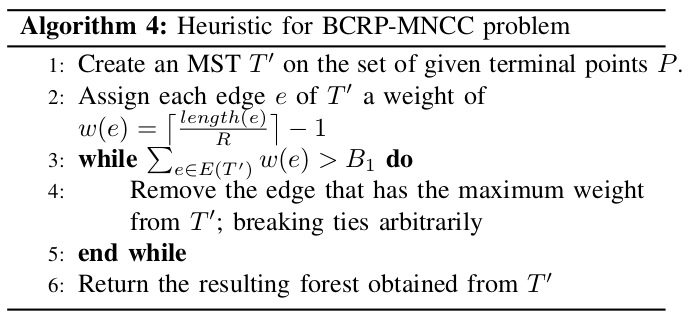
\includegraphics[width=0.9\textwidth]{Alg4.png}
\label{alg4}
\caption{Algorithm 4 from Mazumder et. al.}
\end{figure}\\
As can be seen in Figure 1, calculating the location of relay-nodes that minimizes the number of components utilizes iterative reduction of a minimum spanning tree (MST).
A minimum spanning tree returns the shortest possible way of connecting all the vertices of the graph.
In an ideal case, this minimum spanning tree would provide us a solution to how to place our relay nodes with a single connected network.
However, this is not possible in all cases.
In conditions with limited resources connecting all components may not be feasible.
The algorithm introduces the concept of a budget as an upper limit, where the cost being minimized is a ratio of the euclidean distance and the communication range for a relay node.
Since we are operating on a minimum spanning tree at first and on minimally-connected components in subsequent iterations, removing a single edge results in the creation of an additional component.
We remove the largest cost edges in the tree necessary to fall under our budget, resulting in the minimum number of edges being removed.
In this way, we minimize the number of connected components.\\

\subsubsection*{Second Solution}
To maximize the size of the largest connected component of $G^\prime$, the paper introduces the \textbf{\textit{Budget Constrained Relay node Placement with Maximum size of Largest Connected Component (BCRP-MLCC)}} algorithm.
Given the location of $n$ sensor node locations $P=\{p_1, \hdots, p_n\}$, a communication range $R$, a constant $C$ and budget $B_2$, we can find a subset of $B$ locations $Q=\{q_1, \hdots, q_{|B|}\}$ to deploy relay-nodes such that the size of the largest connected component in the graph $G^\prime=(V^\prime, E^\prime)$ is at least $C$.
The algorithm is given as follows.
\begin{figure}[h]
\centering
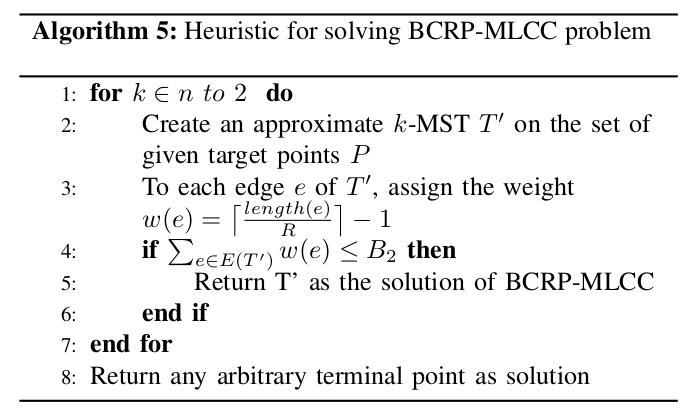
\includegraphics[width=0.9\textwidth]{Alg5.png}
\label{alg5}
\caption{Algorithm 5 from Mazumder et. al.}
\end{figure}\\

To determine the locations of relay-nodes that maximizes the size of the largest connected component, we find the largest approximate minimum spanning tree that comes under budget.
To do this we implement a k-minimum spanning tree (k-MST) approximation.
The k-MST problem is to find a minimum spanning tree of k vertices and is NP-Hard, but many approximations with varying bounds exist.
Note that the output of a k-minimum spanning tree algorithm with $k = \left|V\right|$ would be equivalent to the MST algorithm.
In this implementation we iteratively decrement the value of k from the number of vertices in the graph n to a minimum of two.
With each k, we calculate the k-MST.
If the resulting MST is under budget, that tree is returned as the largest possible component under budget.
Else, we continue with a decremented value for k.
By returning the first approximate MST to fall under this budget we maximize the single connected component size.

\section{Implementation of The Algorithms}
We chose to implement this project in Clojure for several reasons, but particularly the spiritual enlightenment attained from working with graphs and trees from within a language whose source is itself directly manipulated as a tree.
Tying into this, Clojure has a well-defined protocol for graph operations called Loom, enabling us to choose any of the various Loom implementations based on their ergonomics.
Since we knew we would be implementing algorithms from the graph primitives provided by Loom and any implementation thereof, these ergonomics were of particular importance.
For instance, implementing both algorithms described above requires the calculation of minimum spanning trees.
More over, this project was an opportunity to learn more about how lisp-like languages are written and learn the lispy way of approaching problems.
\subsection{BCRP-MNCC}
In the first case, Algorithm 4 from the paper, this is a standard fully spanning tree, while the next algorithm requires minimal spanning trees.
The main benefits of Clojure for our implementation in this case are two-fold: a base protocol that would allow us to swap implementations later if we ran into teething issues with our initial choice of implementation and maximum code flexibility which allows us to wrap any unwieldy aspects of library APIs with minimal effort.

An important part of our implementation has been our use of a disjoint-set library in the process of computing minimum spanning trees, which leans heavily on the disjoint set data structure.
We weren't sure if this was something we were expected to implement ourselves for this algorithm, so we implemented a set of lightweight wrapper functions to allow swapping this library out for an implementation of our own if that turns out to be required.

These well-designed abstractions allow us to implement the required algorithms with minimal cognitive overhead and with our code neatly mapping onto the psuedocode given in the paper.
For example, compare the following code snippet to Figure 1:

\begin{lstlisting}{clojure}
(defn algorithm4
  [graph comm-range budget]
  (let [mst      (minimum-spanning-tree graph)
        weighted (atom (weight-tree mst comm-range))]
    (while (> (total-edge-weight @weighted)
              budget)
      (swap! weighted
             remove-edge
             (max-edge-by @weighted :weight)))
    @weighted))
  \end{lstlisting}

\subsection{BCRP-MLCC}

For Algorithm 5 from the paper, the most difficult portion was the k-MST approximation.
Selecting a k-MST implementation was challenging.
All k-MST implementations have a large time complexity, being approximations for an NP hard problem.
Our goal was to find an implementation which would not dramatically slowed our program.
However, the k-MST implementations with fairly low complexities were far more complicated.
In the end, the more complicated but faster implementation won out and we implemented the k-MST algorithm defined by Garg in \cite{Garg1997}.

The Garg approximation works for items in the Euclidean plane, which is the same limitation for algorithm 5 and is thus a valid implementation.
The approximation works by dividing the space the points inhabit into cells and trying to find as many of the $k$ points from adjacent cells as possible.
By repeatedly breaking into smaller and smaller cells, we find the set of k nodes which lie in the smallest possible cell and use this to form our k-minimum spanning tree.

Suppose we have a graph with a set of points $P$.
For each pair of two points $p_i, p_j \in P$ where P is the set of sensor locations derive the euclidean distance $d(i,j)$ and midpoint $m$.
From these, form a circle centered at $m$ with diameter $\sigma = \sqrt{3}d(i,j)$.
Note that if $p_i$ and $p_j$ are the furthest points from one another all points will be contained in the resulting circle.
The approximation of this circle is merely to find the region in space which we are interested.
Circumscribe the aforementioned circle with a square $Q$ that shares the same center and edge length of $\sigma = \sqrt{3}d(i,j)$, same as the circle diameter.
The purpose behind squaring this circle is to develop a structure that is simple to subdivide.
Our goal is to find $k$ points that are as near to one another as possible.
To do this, we divide the square into quarters, recursively, to produce a grid.
Our base case is when the edge of the cell is less than or equal to the ratio circle diameter $\sigma$ to our number of desired points, or $\frac{\sigma}{k}$
Simply minimizing the number of grid squares the k-MST spans is insufficient, however, as two grid cells may be located in opposite corners of $Q$ and a smaller tree may exist.
To tackle this issue, Garg introduces a potential function for a set of points to determine their proximity.
The potential of a set of points $S$ for a grid $G_i$ with cells of size $x_i$ is designated $G_i(S)$ and equal to $x_it_i$ where $t_i$ is the number of cells in $Q$ containing points of $S$.
This relationship means the potential is minimized in smaller cells.
The minimum potential for our fixed goal of $k$ points will occur in the smallest cell size possible.

The size of the smallest grid size is $x_0 = \frac{\sigma}{k}$  where $\sigma$ is the square edge length and $k$ is the number of points in our desired minimum spanning tree.
Further grid sizes $x_i = 2^ix_0$ for $i > 0$.
At $i = \log k$, $x_i = \sigma$ or the edge size of the square.
Thus the depth of our tree of partitions will have a logarithmic relationship to the number of points in our k-MST.
The total potential for a set of points $S$ is the sum of $G_i$ potentials for this range.
That is, $P(S) = \sum_{i=0}^{\ceil{\log k} - 1} G_i(S)$.

The full k-MST simply iterates over each possible combination of points $p_i$ and $p_j$, creates the circle at the midpoint between them with diameter $\sqrt{3}d(i,j)$, calculates the $k$ points in this circle with the minimum potential, and selects the tree for the $p_i$ and $p_j$ with the lowest total weight.
This algorithm can be seen below in Figure 3.

\begin{figure}[h]
\centering
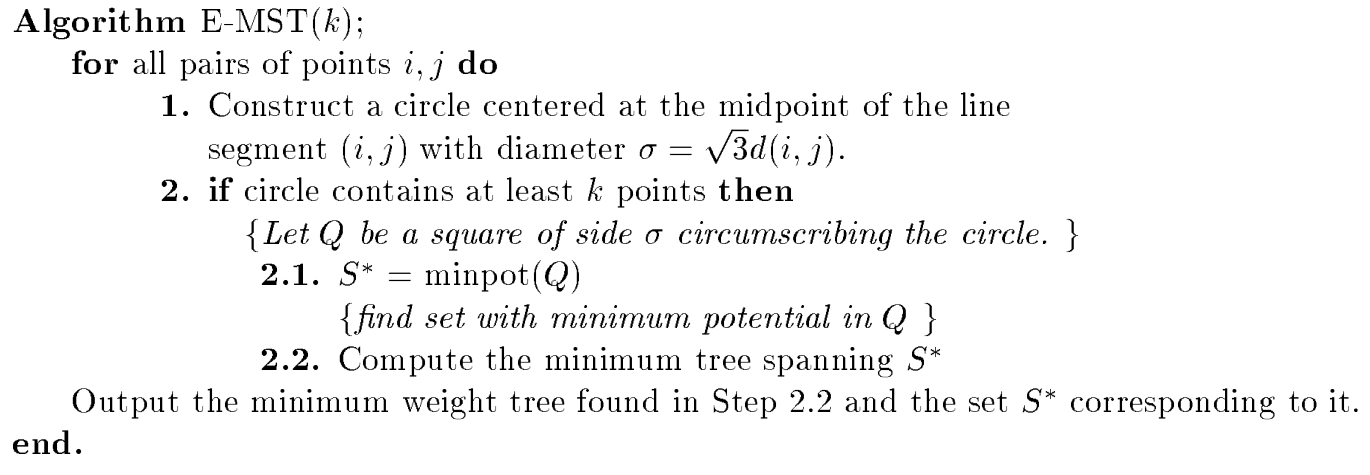
\includegraphics[width=0.9\textwidth]{k-mst.png}
\label{k-MST}
\caption{k Minimum Spanning Tree from Garg 1997}
\end{figure}\\

Our implementation of this algorithm is as follows.

\begin{lstlisting}{clojure}
(defn k-min-spanning-tree
  [graph k]
  (->> (for [[src dst] (get-edges (uber/nodes graph))]
         (let [[mid diameter] (apply get-circle
                                     (map (partial node-location graph)
                                          [src dst]))
               state          {:graph graph :center mid :diameter diameter :k k}]
           (-> state
             minpot
             (get k)
             :points
             (->> (into #{})
               (induced-subgraph graph))
             minimum-spanning-tree)))
    (filter #(= k (count (uber/nodes %))))
(apply min-key total-edge-weight)))
\end{lstlisting}

Once this algorithm was implemented, we could make a fairly exact duplicate of algorithm 5 from the paper.
Our final implementation can be found below.


\begin{lstlisting}{clojure}
(defn algorithm5
  ([graph comm-range budget]
   (algorithm5 graph comm-range budget (uber/count-nodes graph)))
  ([graph comm-range budget k]
   (let [kmst     (k-minimum-spanning-tree graph k)
         weighted (weight-tree kmst comm-range)]
     (if (> (total-edge-weight weighted) budget)
     (recur graph comm-range budget (dec k))
     weighted))))
\end{lstlisting}

\section{Result}
TODO

\section{Conclusion}
This project discusses and implements two algorithms designed to make placement decisions for sensor relay nodes in a limited budget environment.
We implement algorithms that perform this placement while using either number of components or largest component as a placement metric.
These algorithms are the \textit{Budget Constrained Relay node Placement with Minimum Number of Connected Component (BCRP-MNCC)} and \textit{Budget Constrained Relay node Placement with Maximum size of Largest Connected Component (BCRP-MLCC)} respectively.
The BCRP-MNCC is written and has produced excellent results.
We are able to find the optimal placement for nodes on with arbitrary locations, communication range, and budget.
Proof of its functionality can be found above in our results section.
We also have had success with our BCRP-MLCC implementation.
We have a working k-MST approximation that enables us to find, using the algorithm from the paper, the largest connected tree for node placements.
The results of this algorithm are not guaranteed to be optimal given that a true k-MST implementation is NP-Hard, however our approximation is producing reasonable output in our testing.
These resutls can be seen above in the results section.

\section{Peer Review}
Below is the table of all members of our team, scored out of 20.
Note names are in alphabetical ordering.
TODO Fill out table.
\begin{center}
  \begin{tabular}{|c|c|}
     \hline
  Name & Score ($\frac{}{20}$)\\
   \hline
  Zackary Crosley & ? \\
   \hline
  Maxfield Lehman & ?\\
   \hline
  Zahra Zahedi & ?\\
                  \hline
\end{tabular}
\end{center}

\subsubsection*{Zackary Crosley}
TODO Write out eval.
\subsubsection*{Maxfield Lehman}
TODO Write out eval.
\subsubsection*{Zahra Zahedi}
TODO Write out eval.

\bibliographystyle{plain}
\bibliography{references}
\end{document}
